\mcchap{Le dashboard}{cap:dashboard}

\noindent In questo capitolo verranno presentati alcune catture di schermata estratte dalle dashboard.

\section{Dashboard italia}
Nella dashboard Italia vengono rappresentati i grafici che riassumono la situazione della pandemia in Italia

\subsection{Nuovi casi}
Il grafico nella figura \ref{fig:nuovi_casi} mostra l'andamento giornaliero delle nuove persone che risultano positive  al Covid-19.
\begin{figure}[htp]
    \centering
    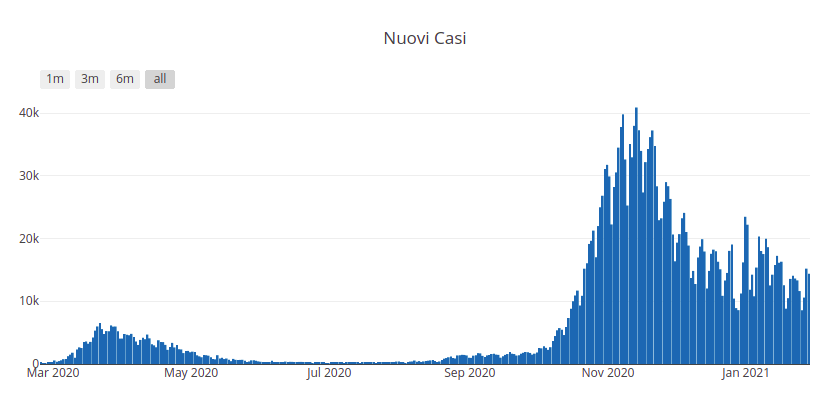
\includegraphics[width=8cm]{nuovi_casi}
    \caption{Nuovi casi}
    \label{fig:nuovi_casi}
\end{figure}

\subsection{Totale casi}
Nella figura \ref{fig:totale_casi}
\begin{figure}[htp]
    \centering
    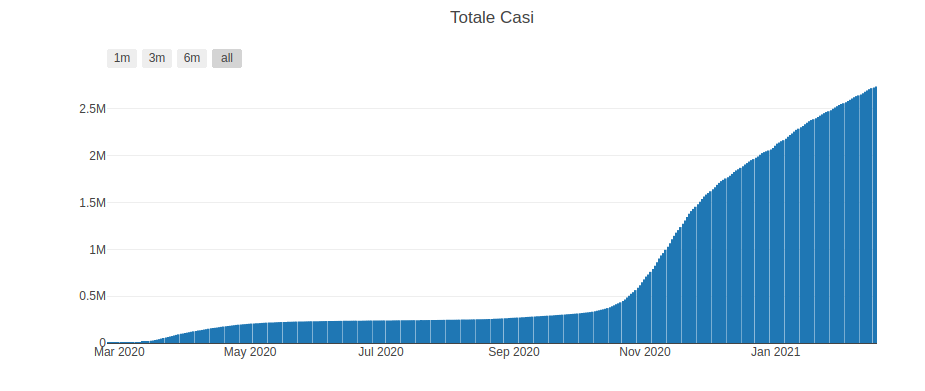
\includegraphics[width=8cm]{totale_casi}
    \caption{Totale casi}
    \label{fig:totale_casi}
\end{figure}

\subsection{Isolamento domiciliare}
Nella figura \ref{fig:isolamento_domiciliare} è raffigurato il grafico delle persone che sono in isolamento presso il loro domicilio.
\begin{figure}[htp]
    \centering
    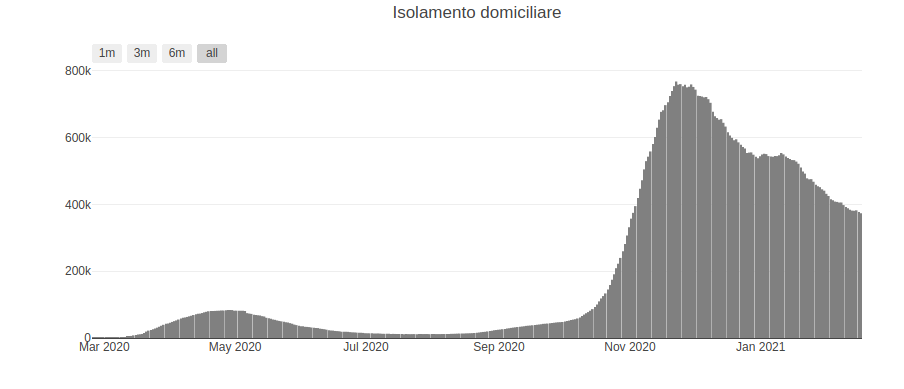
\includegraphics[width=8cm]{isolamento_domiciliare}
    \caption{Isolamento domiciliare}
    \label{fig:isolamento_domiciliare}
\end{figure}

\subsection{Terapia intensiva}
Il grafico della figura \ref{fig:terapia_intensiva} mostra l'andamento dei pazienti ricoverati in ospedale in terapia intensiva.
\begin{figure}[htp]
    \centering
    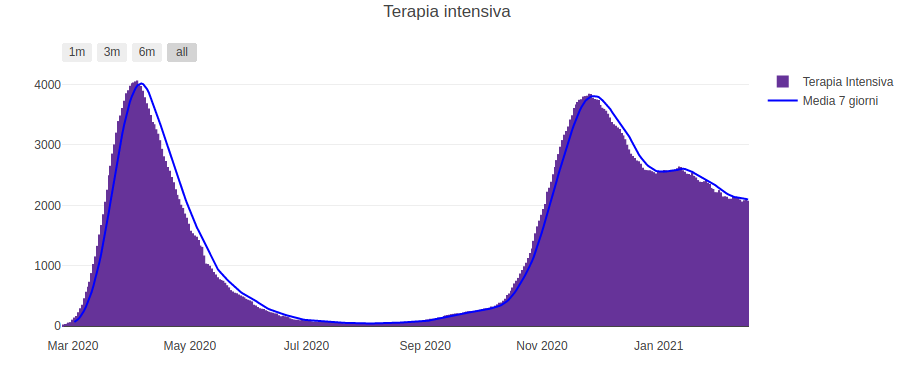
\includegraphics[width=8cm]{terapia_intensiva}
    \caption{Terapia intensiva}
    \label{fig:terapia_intensiva}
\end{figure}

\subsection{Casi normalizzati}
Il grafico nella figura \ref{fig:casi_normalizzati} mostra il numero di casi normalizzati, ossia resi indipendente dai tamponi effettuati ogni giorno.
Si può anche osservare (in arancione) la linea della media mobile a 7 giorni.
\begin{figure}[htp]
    \centering
    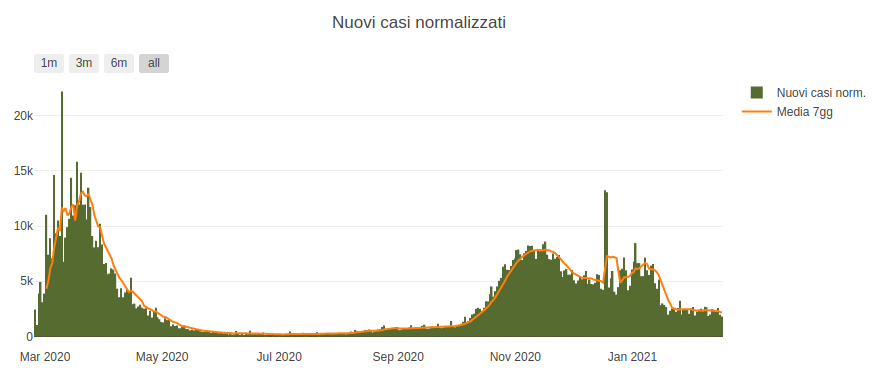
\includegraphics[width=8cm]{casi_norm}
    \caption{Casi normalizzati}
    \label{fig:casi_normalizzati}
\end{figure}


%\section{Dashboard Lombardia}

%\section{Dashboard Regioni}

